\documentclass[conference]{IEEEtran}

\usepackage{authblk}
\usepackage[ruled,algosection,noend,linesnumbered]{algorithm2e}
\usepackage{amsmath}
\usepackage{amsthm}
\usepackage{amsfonts}
\usepackage{subcaption}
\usepackage{tikz}
\usepackage{cite}
\usepackage{graphicx}
\usepackage{adjustbox}
\usetikzlibrary{calc, automata, chains, shapes, snakes}

\newtheorem{privdef}{Privacy Definition}
\newtheorem{secthm}{Security Theorem}

\newcommand{\raphael}[1]{\textcolor{blue}{Raphael: #1}}
\newcommand{\george}[1]{\textcolor{green}{George: #1}}

\begin{document}

\author{Raphael R. Toledo}
\author{George Danezis}

\affil{University College London }

\title{Mix-ORAM,\\ towards a delegated shuffle amortization.}
%what matters the most ? The sorting algo or the use of mixnets ?

\maketitle

\begin{abstract}
{Oblivious RAM systems suffer of impracticality, notably due to the cost of the randomization process in the eviction phase.
We present in this paper an ORAM system relying on amortizable shuffle and mixnet technologies to make it more usable.}
\end{abstract}

\section{Introduction}
\iffalse
\begin{itemize}
 \item Introduction to ORAM (we have to hide the access pattern) ~/
 \item Different ORAM over time \raphael{p.2 TODO}
 \item Eviction is too costly to happen at once /
 \item Emergence of A.S. \raphael{TODO}
 \item Combining ORAM and AS \raphael{p.3 TODO}
\end{itemize}
\fi

Cloud technologies provide a range of services using remote servers, including website hosting, computation, and data storage. One of the main issues for the storage providers is to ensure the users that the data is protected, not only from external adversaries but also itself, and doing so for reasonable costs. 
Cryptographic functions are thus used among other things to create secure communication channels, authenticate users, encrypt and check the data integrity.
These solutions however do not prevent the leakage of some information and its interception. One can for instance count the number of packets exchanged by two parties, even when using anonymity systems \cite{murdoch2005}, and guess which file was accessed thanks to a-priori knowledge (the file size distribution, the file access frequency distribution, etc.).
We can illustrate how much of a problem this is by considering the following example. Eve was recently made redundant by its company which is outsourcing its data to Eve's new workplace. Eve can evesdrop the storage servers and thus observe which files are being retrieved. She may not know the current content of the files but can guess what project they correspond to. Seeing which project is active, she can sell the information to a competitor.  

Oblivious RAM (ORAM)~\cite{goldreich87}, or Oblivious Storage (OS)~\cite{boneh2011}, are key technologies to answer such problem. The access methods are made independent of the sought records to hide the access pattern and the datablocks are periodically randomized to hide which records were previously retrieved.
Improvements have been made on the data retrieval costs thanks to structural change in the data representation, considering trees~\cite{} or rings~\cite{}, and the shuffling algorithm, in particular with the introduction of dummies ~cite{}.
The eviction problem however remains challenging as the whole database has to be reencrypted and sorted again frequently. The database is consequently unreachable for long periods of time during which the user does heavy computing.
In 2013, Stefanov and Shi~\cite{stefanov2013} proposed a multi-cloud oblivious storage where the eviction algorithm was delegated thanks to the use of several semi-trusted clouds. However, the practicality of owning and managing more than one cloud was not discussed in the paper.

Mixing networks is a solution widely applied in Anonymity system to obliviously shuffle packets which could be used here. A batch of packets is received by the mixnet where it is reencrypted and shuffled by each mix such that the output of one mix is the next ones's input. For the adversary to link the input and output, all of the mixes used in the shuffling have to be compromised.
Mixnets could thus address ORAM constraints but at high cost since the reencyption cost is multiplied by the number of mixes. If using mixnet, methods to amortize the shuffle have to be taken into account to make ORAM workable.

\subsection{Our contributions}
In this work, we focus on the eviction algorithm. We present a new security definition for the oblivious sorting algorithm and suggest to leave the eviction and shuffling to untrusted third parties.
The advantages of such practices are the delegation of the shuffling, the possibility to delay the latter to quieter times and the independence from centralized parties.

\begin{itemize}
 \item We present the first ORAM relying on a mixnet for the eviction process.
 \item We give a new security definition of ORAM's eviction. %indistiguishability between accessed and unretrieved elements
 \item We present an amortizable shuffle.
\end{itemize}

\subsection{Content}
After presenting the related work, the ORAM model, its associated threat model and explaining the different costs in Section.~\ref{section1}, we introduce Random Transposition Shuffles, how to use them in ORAM and together with a mixnet and discuss of various optimizations in Section.~\ref{section2}.
We finally evaluate our schemes with standard ORAM model and discuss about the advantages and drawbacks of using mixnets.


\section{Preliminaries}
\label{section1}

\subsection{Related Work}
\subsubsection{ORAM}
% first ORAM square-root, partition Trees Rings

\subsubsection{Shuffling and Sorting.}

%diff sorting/shuffling (knowledge of the output permutation)
\noindent\textbf{Shuffling}
\iffalse
\raphael{Melbourne Shuffle intro for inspiration}
A shuffle is an algorithm for rearranging an array to achieve a random permutation of its elements.
Early shuffle methods were motivated by the problem of shuffling a deck of cards.
Classic card shuffle methods(e.g.,Knuth(orFisher-Yates)[17],the riffle shuffle[2],Thorp shuffle[24]) are not data-oblivious, however, as anyone observing card swaps or riffles (interleaving two subdecks) of such methods can learn the final output permutation.
In ICALP 2012, Goodrich and Mitzenmacher [10] showed that one can,in fact,shuffle a deck of n cards and guarantee that an observer cannot find a particular card in the output permutation with probability better than O(1/n).
However, this algorithm is not an effective shuffle for our purposes,since the output permutations produced by the algorithm are not allequally likely and there may be dependencies between large groups of cards that could be leaked.
Most other existing efficient data-oblivious shuffling methods assign random values to the elements of the array and use a dataoblivious algorithm to sort the array according to these values.
\fi
\noindent\textbf{Sorting} \\
%sorting...
%Oblivious sorting: - sorting networks - Melbourne shuffle

\subsubsection{Mixnets.}
\iffalse
\raphael{from lower PIR, rewrite, not only cascade, focus on mixing...}
Research on Anonymity Systems (AS) began in 1981 by David Chaum introducing the mixnet for anonymous e-mail \cite{Pseudo}.
Other AS applications were then studied, such as peer-to-peer and web browsing, in particular in the context of Onion Routing and Tor~\cite{DBLP:conf/uss/DingledineMS04}.
The Anonymity System accepts a batch of messages and routes them while hiding the correspondence between senders and receivers.
Low-latency anonymity systems, however, may still fail under attacks such as traffic analysis and fingerprinting~\cite{Fingerprinting}.
Cascade mix networks offer perfect privacy at the cost of lower performance \cite{berthold2001disadvantages}.
In this work we will always consider an ideal anonymity system that can be abstracted, from the perspective of an adversary, as an unknown random permutation of input messages to output messages. Real-world instantiations are imperfect and security parameters may have to be adapted, or in the case of onion routing systems~\cite{DBLP:conf/uss/DingledineMS04} some additional batching and mixing may be required.
\fi

\subsubsection{Differential Privacy.}
\iffalse
\raphael{May be erase. If not, rewrite, add lower cost...}
Differential Privacy definitions and mechanisms were first presented in 2006~\cite{DiffPrivacy} to enable safe interactions with statistical databases.
However, this definition has since been used in machine learning~\cite{DeepLearning}, cloud computing~\cite{Airavat}, and location indistinguishability together with PIR~\cite{GeoIndis} to evaluate and minimize the privacy risk.
Differentially private definitions have several advantages: they capture the intrinsic loss of privacy due to using a mechanism, and they are not affected by side information the adversary may hold.
Well-known composition theorems can be applied. We note that Chor et al.~\cite{Chor} also make passing allusion to statistical and leaky definitions of PIR in their seminal paper, only to focus on perfectly information-theoretic schemes.
\fi

\subsection{Model}
We consider on one side, a remote server with memory capacity of $\mathcal{O}\left(n\right)$ $b$-bit long blocks, a cascade mixnet composed of $m$ mixes and on the other side, a client with memory of $s$-block capacity with $s<<n$. 

We consider traditional cloud opertions...
\begin{itemize}
 \item get(index)
 \item get\_range($index_i$, $index_j$)
 \item put(index) 
 \item put\_range($index_i$, $index_j$)
\end{itemize}

\subsection{Threat model}
We consider an adversary $\mathcal{A}$ has corrupted $m_{a}$ mixes and potentially the ORAM database in order to discover the relationship between the user's records and indexes. 
The corrupted servers are said honest but curious in that they perform correctly the assigned protocols and algorithms but passively record and share all information they observe to achieve this objective.
We also assume that the adversary observes all the user's incoming and outgoing communication. However, we assume that all messages, database request or mix packet, are encrypted and that only message timing, volume and size from honest servers are visible to the adversary.
Attacks and countermeasures to such attacks will only be examined in the Discussion section (c.f. Section.\cite{}).

\subsection{Costs}
We denote the communication costs by $C_o$ for the number of \emph{bits} sent by the ORAM, $C_{c}$ by the client, and by $C_{m}$ sent by the mixes. 
We will call $C_p$ the computation cost derived from the eviction and $C_a$ from the database accesses.

\subsection{Cryptographic Primitives}
\begin{itemize}
 \item Encryption 
 \item Seeds \raphael{TODO ?}
\end{itemize}

\section{Mix-ORAM}
\label{section2}
After looking at a simple but impractical mix ORAM we will look closely at the eviction process and the use of shuffle algorithms, we will then apply the result to a traditional client-server ORAM and finally to the mix-ORAM.

\subsection{A simple Mix-ORAM}
%Passing the DB from a mix to another
%Reencryption network thks to AES-CTR commutation property
We consider here the basic case where the whole database is sent through a cascade mixnet during the eviction process as shown in Fig.\ref{fig:ASMO}.
Each of the mixes reencrypts and permutes every record in a way such that the user only has to remember a constant amount of information, that is to say $\mathcal{O}\left ( m \right )$ permutation seeds ($S_i$) and encryption keys ($k_j$).

To do so, because the symmetric group is not commutative, the mixes first undo the previous permutation (executing $\Pi_{S_m^{-1} \circ .... \circ S_1^{-1}}$) before sorting the records (executing $\Pi_{S_1' \circ .... \circ S_m'}$) to the new ordering.We also consider reversing the mixnet flow during the second step, the records now going from the last mix to the first before being uploaded on the database, to avoid unnecessary communication costs.\\
As for encryption, we use AES-CTR for its speed. Since AES-CTR is stateless and commutative, the reencryption order does not matter.However in order to avoid disclosing the initial order to a potential adversary, we'd rather encrypt the records again before deciphering the previous encryption.\\
The security guarantees rely on the fact that no private information (seed, encryption key) is leaked between innocent mixes and corrupted ones and that the encryption is not deterministic.

Alonside the database records, the user need to send the encrypted seeds and reencryption keys. Hence if we denote by $x$ the size in bits of a seed and encryption key, the total communication cost is of the order $\mathcal{O}\left ( m\cdot N \right )$, more precisely $C_m=2mN + m\cdot(2m-\frac{1}{2})\cdot x$.
The computation cost is of the order $\mathcal{O}\left(mN\right)$, the encryption process comprising most of it.

This scheme is not efficient as instead of reencrypting each record twice as in the Melbourne Shuffle, $2\cdot m$ encryption per element is necessary to achieve perfect security. The whole database also has to be passed through every node twice which incur severe delays. Parallelization could help increase the efficiency of the mixnet by distributing the workload among mixes, however the cascade configuration would have to change.
We can try to limit the number of seeds and encryption keys the user has to store by reusing some. However doing so, an adversary can discover in some cases, the probability depending on the number of compromised mixes and number of reuse, what permutations or encryptions was done by bruteforcing on a small universe.

\begin{figure*}[t!]
\centering
\begin{adjustbox}{width=\textwidth}
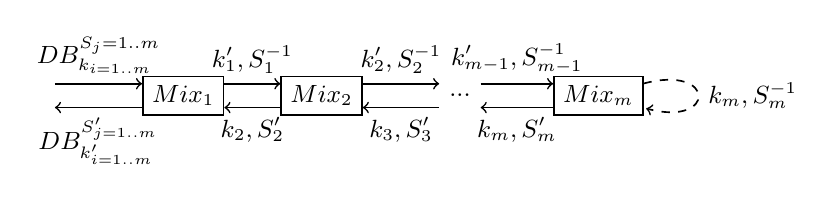
\begin{tikzpicture}[->, auto, semithick,  node distance = 5em, scale=0.5]
\tikzstyle{every state}=[fill=white,draw=black,thick,text=black]
\node[draw=none, fill=none]    		(0)		  {};	
\node[draw, rectangle]   		(A)[right of=0]   {\small$Mix_{1}$};
\node[draw, rectangle]    		(B)[right of=A]   {\small$Mix_{2}$};
\node[draw=none, fill=none]    		(X)[right of=B]   {\small$...$};
\node[draw, rectangle]    		(Z)[right of=X]   {\small$Mix_m$};

\path
([yshift=2ex]0.east) edge     	node{\small$DB_{k_{i=1..m}}^{S_j=1..m}$}    	([yshift=2ex]A.west)
([yshift=-2ex]A.west) edge     	node{\small$DB_{k'_{i=1..m}}^{S'_{j=1..m}}$}    	([yshift=-2ex]0.east)

([yshift=2ex]A.east) edge     	node{\small$k_1',S_1^{-1}$}    	([yshift=2ex]B.west)
([yshift=-2ex]B.west) edge     	node{\small$k_2,S_2'$}    	([yshift=-2ex]A.east)

([yshift=2ex]B.east) edge     	node{\small$k_2',S_2^{-1}$}    	([yshift=2ex]X.west)
([yshift=-2ex]X.west) edge     	node{\small$k_3,S_3'$}    	([yshift=-2ex]B.east)

([yshift=2ex]X.east) edge     	node{\small$k_{m-1}',S_{m-1}^{-1}$}    	([yshift=2ex]Z.west)
([yshift=-2ex]Z.west) edge     	node{\small$k_m,S_m'$}    	([yshift=-2ex]X.east)

(Z)    edge[loop right, dashed]    node{\small$k_m,S_m^{-1}$} (Z);

\end{tikzpicture}
\end{adjustbox}
\caption{A simple Mix-ORAM} \label{fig:ASMO}
\end{figure*} 


\subsection{The Eviction process.}
In this section we present random transposition shuffles (RTS) and argue their use enable the eviction process to be amortized over time.
We first present the mixing time of $k$-RTS before introducing ORAM assumptions to reduce even more the expected time to achieve randomness to the eyes of the adversary.

\subsubsection{$k$-Random Transposition Shuffle.}
% Def of RTS. RTS can be broken down in independant rounds which is nice for amortization. RTS can be made oblivious by making the permutations locally. The mixing time for RTS is high, we look at oblivious k-RTS.
Random Transposition Shuffles (RTS) are widely used examples in the study of card shuffling. It consists in a player picking randomly a couple of cards from a same deck, permuting them according to a coin toss and putting them back at the same location.
These steps, usually called a round, are then repeated until the deck of cards has been properly shuffled, i.e. until every card arranging is possible.
We can already see why RTS are natural candidates for amortized ORAMs : if they can be broke down in independant rounds which can be spread over time, so can a randomization process based on them. Futhermore, having the client (player) permuting the data blocks (cards) locally is enough to make RTS oblivious to the eyes of an adversary.
Diaconis in 19XX~\cite{} has proved that the RTS mixing time of a deck of $n$ cards is of the order of $n\log(n)$. We thus first look at oblivious $k$-RTS, an RTS where the client picks and permutes locally $k$ distinct cards, to make the scheme more efficient.

\begin{secthm}
\textbf{Mixing time of $k$-RTS.} A $k$-random permutation shuffle of a $n$ card game reaches the uniform distribution in $\tau$ rounds, such that
\begin{align*}
E(\tau) &< \frac{2}{k}\cdot\frac{n^2}{n+1}\cdot \left ( \log(n) + \mathcal{O}(1) \right ) &\\
\sigma^2(\tau) &< \frac{4}{3} \cdot {\pi}^2 \cdot \left ( \frac{n}{k} \right )^2 &
\end{align*}
\end{secthm}

An oblivious $k$-RTS implies computation and communication cost of the order of $\mathcal{O} \left(n\cdot \log(n)\right)$.
\raphael{Calculte the exact numbers and compile them in a table.}

\subsubsection{Oblivious Merge}
%Assumption: merge of indistiguishable elements
Before the eviction algorithm is run, the database can be represented as a simple binary array of $n$ bits out of which $s$ are 1s and $n-s$ are 0s. These two sets respectively correspond to records which were accessed (the 1s) or not (the 0s) by the user.
We argue that in this representation, elements of the same sets are indistiguishable to the adversary thanks to prior encryption and permutation.
This simplifing assumption significantly reduces the number of possible orderings in the adversarial view, we can prove, thanks to the Bars and Stripes theorem, that there now are ${n \choose s}$ arrangings instead of $n!$, that is to say a gain of order $\mathcal{O}\left ( (n-s)!\cdot s!\right )$.

We now consider the RTS process in that scenario and suppose the records (the bits) are reencrypted before being permuting such that the merge of the two sets is oblivious to the adversary.

\begin{secthm}
An oblivious merge of 2 indistiguishable sets of respective size $n$ and $s$ requires $\tau$ rounds such that any arranging is possible, with
\begin{align*}
\tau(\epsilon) &\geq \frac{n}{({n \choose s}-1)^{\frac{1}{n-1}}-n} \log\left(\frac{1}{2 \epsilon} \right) &\\
\tau(\epsilon) &\leq \frac{2}{\eta} \left (\frac{1}{s} \right )^2 \cdot \left [ s \left( \log \left (\frac{n}{s-0.5}\right) +\mathcal{O}\left(1\right) \right ) - 2\log \left( 4 \cdot \epsilon\right) \right ] &\\
\tau(\epsilon) &\leq 2 s^2 \left(1- \frac{s}{n} \right )^2 \cdot \log \left(\frac{{n \choose s}}{4\cdot\epsilon^2}\right) \raphael{to\ be\ proved}
\end{align*}
Proof can be found in Annexe.~\cite{}.
\end{secthm}

\subsubsection{Amortizable sort}

We now use the $k$-RTS and Oblivious Merge to create an obivious amortizable sort algorithm. The $k$ parameter is directly linked to the memory and influence the speed of randomization, ideally we have $k=m$.

The user first rerandomizes the elements keeping in memory each of their location (cuckoo hashing?) then reaches a fixed distribution $\pi$ given by a seed.
\raphael{I think we do as this ?}
\raphael{how do we do the permutations? --> what is the format of the seed ? how do we combine them ?}

\subsection{A simple ORAM.}
We consider in this part a traditional ORAM system composed of the client with a memory of $\mathcal{O}\left(\sqrt{n}\right)$ blocks and a remote server with a memory of $\mathcal{O}\left(\sqrt{n}\right)$ blocks which uses our oblivious merge during the eviction process.


\subsection{Eviction process: the Mixnet.}
%Stress that this is a new case for mixnet as the messages come from the same source but the mixnet client/user needs to retain some information about the output.
To evict the stash, the client updates the former in the database and sends a signal to the mixnet or to the database if he wants the eviction to be postponed to quieter times.

Two different methods can be applied for the eviction process depending on the mixnet architecture, in both cases eviction rely on repeatedly fetching $k$ records, refreshing and permuting them before updating them back in the ORAM.
If the mixnet is a cascade network, the first mix outputs the resulting array to next mix while repeating the process for distinct records, otherwise, in the mesh case, the mixes fetch in parallel the records.
The cascade case is more advantageous in time as the outputs and inputs of the mixes coincide, hence the communication cost is roughly divided by two. There is futhermore no synchronization needed between the mixes to process different records at the same time.
However what is gain in duration is loose in resilience as any mix failure in the cascade mixnet would compromise the whole system. Moreover an attack specific to cascade mixnet also needs to be taken into account: if the first mix and the database are both corrupted, the permutation could be done only on a subset of records
so that the adversary knows the positions of a non trivial number of records, as they were not permuted, without the honest mixes and the client realizing it. To counter it, the first mix query should be sent along the records to all the mixes together with an identification proof.

Another problem raises

\raphael{Use of distributive encryption ?}

The computation cost of the eviction would thus be of the order of $m\cdot n \cdot \log(n)$ while the communication cost will be either $4\cdot m \cdot n \log(n)$ or $2\cdot(m+1) \cdot n \log(n)$ depending on the mixnet architecture.

\raphael{Can we delay the encryption ? ($k_{in}=k_{out}$)}

\subsection{Lowering Eviction Costs.}

In order to lower the eviction costs sustained by the mixnet, optimizations on each side of the channel can be done.

\subsubsection{Client Optimization.}
\noindent\textbf{Changing ORAM access.}

The client, to lower the eviction costs, could instead of fetching only the requested record query $k-1$ other dummy records. Doing so, we can advance further towards the uniform distribution before the eviction process, measure the distance between the two distributions and reduce the database shuffling cost by having the mixnet performing cheaper and weaker permutations.
What's more, requesting more records can help in hidding the access pattern to the adversary has discussed in~\cite{Lower cost PIR}.

For instance if $n=10^4,\ k=\log(n)=4$ and the stash has a size of $\sqrt(n)=100$, without considering fake accesses, we need 25 accesses before evicting the stash.\\

\noindent\textbf{Considering fake access.}

When a user wants to access a record which already is in the stash, a random database access is performed to hide potential frequency attacks: an adversary having observed the record access frequency beforehand and knowing the average access per day would be able to guess which records are in the stash by not observing accesses which should happen.
These fake accesses can be considered as free permutations as no fetched records need to remain in the stash, thus we can arbitrarily set $k_{in}=k_{out}$.

\begin{secthm}
In the case of a uniform distribution access we have an average number 0 of fake access for $s<<n$.\\
The proof can be found in the Annexe.~\ref{Annexe:FAccess}
\end{secthm}

However it is well known that the frequency access of records is not uniform.
\begin{secthm}
Let $A$ be the access distribution. Let's call $v_0$ and $v_1$ the volume above the line $y=0$ and under it respectively.
The average number of fake access is $ \frac{v0}{v1}$.
\begin{proof}
 The volume under such line represents the number of real accesses a user does while the volume above it represents accesses in the stash which leads to fake accesses.
 When the number of accesses is great, the access frequency approaches the average number of accesses.
\end{proof}
\end{secthm}

\subsubsection{Mixnet Optimization.}

Instead of requiring the mixes to permute all of the $k$ fetched records, the user could set as a parameter of the system the probability of permuting an element $p=\frac{\alpha}{k}$, with $\alpha$ the average number of records to permute.
In that case, the probability a record's index is known to the adversary can be reduced to the probability a record has not been permuted.

\raphael{Differential privacy ?}
\iffalse
\begin{secthm}
 The probability a record was not permuted is
 \begin{align*}
 \Pr &= \left ( 1 - \frac{\alpha}{k} \right )^{m-m_a} \text{ during one round and,} \\
 \Pr &= \left ( 1 - \frac{\alpha}{k} \right )^{(m-m_a)\log(n)} \text{ for the eviction.}
 \end{align*} 
\end{secthm}
\fi

\section{Evaluation}

\raphael{Check Cost section and columns. Choose techs}

\iffalse
\begin{table*}[t!]
\centering
 \begin{tabular*}{\linewidth}{@{\extracolsep{\ fill}}l|c|c|c|c}
  ORAM 		& Access Overhead 	& Message size			& Client Memory 	& Server Storage	\\ \hline
  Others	&			&				&			&			\\ \hline
  Mix 		& $\mathcal{O}(1)$	& $\mathcal{O}(log(n))$		& $s$			& $\mathcal{O}(n)$			\\ 
  Mix opt	& $k\cdot \log(n)$	& $\mathcal{O}(k\cdot \log(n))$	& $s$			& $\mathcal{O}(n)$					 
 \end{tabular*}
 \captionsetup{justification=centering}
 \caption{System comparison where the online access overhead is the number of accesses to retrieve the requested item.}\label{tab:summarySystem}
\end{table*}
\fi

\section{Discussion}
\begin{itemize}
 \item Ads and Cons of mixnets
 \item Multiuser oram
 \item Using proof of shuffle and proof of work to counter injection attacks.
 \item Using a reputation system alongside to dismiss mixes more quickly.
\end{itemize}

\section{Acknowledgement}
MSR...

\section{Conclusion}
\begin{itemize}
 \item New ORAM with mixnet
 \item amortizable eviction
\end{itemize}


\bibliography{mix_oram}{}
\bibliographystyle{plain}

\appendix 
\section{Proofs of Theorems}

\subsection{Proof of Permutation ORAM}
\subsubsection{Proof of k permutation}
\begin{proof}
To first prove the upper bound and variance, we use Diaconis\cite{} results which states that $\tau$ defined in the following game is a strong stationary time.
In a random transposition shuffle, the cards chosen by the right and left hands at time $t$ are respectively called $R_t$ and $L_t$. Assuming that when $t=0$, no card is marked, we mark $R_t$ if
$R_t$ was unmarked before and either $L_t$ is marked or $L_t = R_t$. The variable $\tau$ represents the time when every card has been marked, we call it the stopping time.

Let be $\tau_t$ the number of transpositions after the $t^{th}$ card is marked, up to and including when the $(t+1)^{th}$ is marked. $$\tau = \sum_{i=0}^{n-1} \tau_i$$.
The $\tau_t$ are independant geometric variables with probability of success $p_t$ as implied by the game rules.
The probability of success corresponds to the probability of marking at least one card, one to $t$ cards exactly. To do so, the right cards must be chosen from the unmarked set, comprising $n-t$ cards at time $t$,
and the left cards from the union of the marked set and the right cards.
\begin{align*}
 p_t &= \sum_{i=1}^{min(k,n-t)} {k \choose j} \cdot \frac{ {t+j \choose j} \cdot {n-t \choose j} }{ {n \choose j}^2 }&\\
 &= k \frac{(t+1)\cdot(n-t)}{n^2} + \sum_{i=2}^{min(k,n-t)} {k \choose j} \cdot \frac{ {t+j \choose j} \cdot {n-t \choose j} }{ {n \choose j}^2 }&\\
 &= k \frac{(t+1)\cdot(n-t)}{n^2} + \alpha_{n,t,k} \text{ with } 0 \leq \alpha_{n,t,k} \leq 2^t
\end{align*}

We can thus rewrite $\tau$'s expectation as following.
\begin{align*}
 E(\tau) &= \sum_{t=0}^{n-1} \frac{1}{p_{t}} &\\
 &= \sum_{t=0}^{n-1} \frac{n^2}{k \cdot (t+1)\cdot(n-t) + \frac{\alpha_{n,t,k}}{n^2}}&\\
 &< \sum_{t=0}^{n-1} \frac{n^2}{k \cdot (t+1)\cdot(n-t)}  &\\
 &< \frac{1}{k} \cdot \frac{n^2}{n+1} \cdot  \sum_{t=0}^{n-1} \left ( \frac{1}{t+1} + \frac{1}{n-t} \right ) &\\
 &< \frac{2}{k} \cdot \frac{n^2}{n+1} \cdot \sum_{t=1}^{n} \left ( \frac{1}{t} \right ) &\\
 &< \frac{2}{k} \cdot \frac{n^2}{n+1} \cdot H_n  < \frac{2}{k} \cdot \frac{n^2}{n+1} \cdot \left( \ln(n) + \gamma +\mathcal{O}(\frac{1}{2n}) \right )&\\
 \text{ with } \gamma &= \lim_{n \to \infty} \left ( H_n - \ln(n) \right ) & \\
 \end{align*}
 \begin{align*}
 var(\tau) &= \sum_{t=0}^{n-1}\frac{1-p_t}{{p_t}^2}\ <\  \sum_{t=0}^{n-1}\frac{1}{{p_t}^2} &\\
 &< \sum_{t=0}^{n-1}\frac{1}{\left ( k \frac{(t+1)\cdot(n-t)}{n^2} + \alpha_{n,t,k}\right )^2}\ <\ \sum_{t=0}^{n-1} \frac{1 }{\left ( k \frac{(t+1)\cdot(n-t)}{n^2} \right )^2} &\\
 &< \frac{n^4}{k^2} \left ( \sum_{t=0}^{\frac{n}{2}-1} \frac{1}{\left ( (t+1)(n-t)\right )^2}  + \sum_{t=\frac{n}{2}}^{n-1} \frac{1}{\left ( (t+1)(n-t)\right )^2} \right ) &\\
 &< 2 \cdot \left (\frac{n}{k} \right )^2 \cdot \left (\frac{n}{n/2} \right )^2 \cdot \sum_{t=0}^{n/2-1} \frac{1}{(t+1)^2} &\\
 &< \frac{4}{3} \pi^2 \cdot \left (\frac{n}{k} \right )^2 
\end{align*}
\\

To now prove the lower bound of $\tau$, we will compare the number of fixed points of a permutation $\sigma$, $F(\sigma)$, for our shuffle, the permutation
obtained from the identity by applying $kt$ random transpositions $ P^{kt}(id, \cdot)$, and the uniform distribution $\pi$, or more precisely compare the corresponding probabilities over the set $A=\{\sigma : F(\sigma) \geq \frac{\mu}{2} \}$.
We can say that after $t$ shuffles, the number of untouched cards of our shuffle has the same distribution as the number $R_{2kt}$ of uncollected coupon types after $2kt$ steps of a coupon collector chain
and that about $ P^{kt}(id, \cdot)$ that the associate $F(\sigma)$ is at least as large as the number of cards that were touched by none of the transpositions, i.e. $P^{kt}(id,A) \geq P(R_{kt}\geq A) $.

We know that the $R_{2kt}$ has expectation $\mu = np$  with $p=\left ( 1 - \frac{1}{n} \right )^{2kt}$, variance $var = np(1-p) <\mu$ and by Chebyshev, we know that $\Pr(R_{2kt}\leq \frac{\mu}{2})\leq \frac{4}{\mu}$
as $\Pr(|R_{2kt} - \mu|\geq \frac{\mu}{2}) = \Pr(R_{2kt} \geq \frac{3\mu}{2}) + \Pr(R_{2kt} \leq \frac{\mu}{2}) > \Pr(R_{2kt} \leq \frac{\mu}{2})$.\\

By Markov's inequality we know that $\pi(A) \leq \frac{2}{\mu}$.\\

As $P^{kt}(id,A) \geq P(R_{kt}\geq A) $, we also have $P^{kt}(id,A^c) \leq P(R_{2kt}\leq A) \leq \frac{4}{\mu} $ which leads to $P^{kt}(id,A)\geq1 - \frac{4}{\mu}$.\\

Thus we have $d(t)=||P^{kt}(id,) - \pi ||_{TV} \geq |1 - \frac{4}{\mu} - \frac{2}{\mu}| \geq 1 - \frac{6}{\mu}$.\\

We want to find the minimum $t$ such that $1-\frac{6}{\mu}\geq \epsilon$, which is equivalent to $n \cdot \left ( 1 - \frac{1}{n} \right )^{2kt} \geq \frac{6}{1-\epsilon}$ and to
$$\log\left(\frac{n\cdot (1-\epsilon)}{6}\right) \geq 2kt \log \left ( \frac{n}{n-1} \right )$$
As $\log(1+x) \leq x$, the previous inequality holds if $\log\left(\frac{n\cdot (1-\epsilon)}{6}\right) \geq   \frac{2kt}{n-1} $ which means that if $t\leq \frac{n-1}{2k}\cdot \log\left ( \frac{n(1-\epsilon)}{6}\right )$ then $d(t)\geq \epsilon$.
Thus,
$$\tau \left (\epsilon \right ) \geq \frac{n-1}{2k} \ln(n\cdot \frac{1-\epsilon}{6}) $$.
\end{proof}
\subsubsection{Proof of fake accesses}
\label{Annexe:FAccess}
\begin{proof}
 We want to prove that the average number of fake access is 0 in case of a uniform distribution. To do so, we consider the markov chain in Fig~\ref{fig:AMC} and its Transition Matrix as depicted in Fig~\ref{fig:ATM} for $s=5$.
 \iffalse
\begin{figure*}[t!]
\centering
\begin{adjustbox}{width=\textwidth}
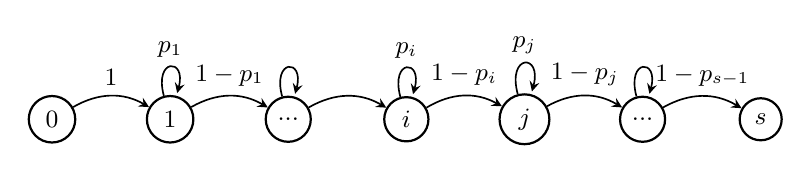
\begin{tikzpicture}[->, >=stealth, auto, semithick, node distance=1.5cm]
\tikzstyle{every state}=[fill=white,draw=black,thick,text=black,scale=1, minimum size = 1em]
\node[state]    (A)               {\small$0$};
\node[state]    (B)[right of=A]   {\small$1$};
\node[state]    (x)[right of=B]   {\small$...$};
\node[state]    (i)[right of=x]   {\small$i$};
\node[state]    (j)[right of=i]   {\small$j$};
\node[state]    (y)[right of=j]   {\small$...$};
\node[state]    (D)[right of=y]   {\small$s$};
\path
(A) edge[bend left]     node{\small$1$}     (B)
(B) edge[bend left]     node{\small$1-p_1$}     (x)
    edge[loop above]    node{\small$p_1$}       (B)
(x) edge[bend left]     node{}     (i)
    edge[loop above]    node{}       (x)
(i) edge[bend left]     node{\small$1-p_i$}     (j)
    edge[loop above]    node{\small$p_i$}       (i)
(j) edge[bend left]     node{\small$1-p_j$}     (y)
    edge[loop above]    node{\small$p_j$}       (j)
(y) edge[bend left]     node{\small$1-p_{s-1}$}   (D)
    edge[loop above]    node{} (y);
\end{tikzpicture}
\end{adjustbox}
\caption{Access Markov Chain, with $p_i=\frac{i}{n}$} \label{fig:AMC}
\end{figure*} 

\begin{figure}
\[
\begin{bmatrix}
         0 & 1      &        &            &         &\text{\huge0}        \\
         0 & p_1    & 1-p_1  &            &         &        \\
          &        & p_2    & 1- p_2     &         &        \\
          &        &        & 1- p_{3} & p_{3} &        \\
          &        &        &            & p_4     & 1-p_4  \\
          &\text{\huge0}        &        &            &        & 1
\end{bmatrix}
\]

\caption{Corresponding Transition Matrix $P$, for $s=5$} \label{fig:ATM}
\end{figure}
\fi
The transition matrix $P$ represents the $s$ transient state, in which the stash is not completely filled, and the absorption state in which the stash is full.
Thus, $P$ can be decomposed in 4 submatrices: the square submatrix $Q_s$ representing all the transcient state, the column matrix R with the probabilities of transitioning to the absorbing state, the null row matrix and the absorption matrix.
\[
\begin{bmatrix}
   Q_s & R \\
   0_{1\times s}   & I_1 \\
\end{bmatrix}
\]
To find the average number of steps from one state to the absorbing one, we have solve the following equation, each row corresponding to the average number of steps from the corresponding state (the stashed filled with some records) to the state where the stash is full.
\begin{align*}
 t &= \left (\sum_{k=0}^{\infty} {Q_s}^k \right ) 1 \\
   &= (I_s -Q_s )^{-1} 1
\end{align*}
This equation has a solution since $M=I_s -Q_s$ have independant rows and thus an inverse that we call $N$.
By calculus we find that,
\begin{align*}
 n_{i,j} &= 0 &\text{ if } i>j,\\ 
 n_{i,j} &= \frac{1}{m_{i,i}} &\text{ if } i=j,\\
 n_{i,j} &= - n_{i+1,j } \cdot \frac{m_{i,i+1}}{m_{i,i}} &\text{ if } i<j 
\end{align*}
which can be simplified by
\begin{align*}
 n_{i,j} &= 0 &\text{ if } i>j,\\ 
 n_{i,j} &= \frac{1}{m_{j,j}} \prod_{k=1}^{j-1} \left ( - \frac{m_{i,k+1}}{m_{k,k}}\right ) &\text{ if } i\leq j
\end{align*}
We only want to calculate the first solution $S_1$ from the equation.
\begin{align*}
 S_1 &= \sum_{j=0}^{s-1} \frac{1}{m_{j,j}} \prod_{k=1}^{j-1} \left ( - \frac{m_{i,k+1}}{m_{k,k}}\right ) \\
     &= \sum_{j=1}^{s-1} \frac{1}{m_{j,j}} \text{ as } m_{i,k+1}= -m_{k,k} \\
     &= \sum_{j=0}^{s-1} \frac{1}{1-\frac{j}{n}} = \sum_{j=0}^{s-1} \left (1 + \frac{j}{n-j} \right ) \\
     &= s + \sum_{j=0}^{s-1} \frac{j}{n-j} \\   
\end{align*}
As $s$ steps are required to fill the stash, we thus find the following inequality for the number of fake access $f$:
$$ \frac{s \cdot (s+1)}{2 \cdot n} < f < \frac{s \cdot (s+1)}{2 \cdot (n+1-s)} $$


\end{proof}

\subsubsection{Proof of Oblivious Merge}
\label{proofOM}

We want to find the mixing time $\tau(\epsilon)$ of our oblivious merge of two sets of indistinguishable elements. To do so, we use the bound of the mixing time of an irreducible ergodic Markov Chain, where $p = \frac{1}{|V|}$ and $1-\lambda^*$ is the spectral gap,
$$\frac{\lambda^*}{1-\lambda^*} \cdot \log\left(\frac{1}{2 \epsilon} \right)\leq \tau(\epsilon) \leq \frac{1}{1-\lambda^*}\cdot \log \left( \frac{1}{2 \epsilon \cdot \sqrt{p}}\right) $$

We now want to find a bound for $\lambda^*$. We represent the arranging of merge of the 2 distinct sets by $\mathcal{G}$, a $k$-regular bipartite graph with $v$ vertices corresponding to the different arrangings and the undirected edges to transpositions of two elements.
By definition, the eigenvalues of the transition matrix of the $\mathcal{G}$ are $k={\lambda'}_0 > {\lambda'}_1 \geq  ... \geq {\lambda'}_{n-1}$, and we have,
$$\text{diam}\left( \mathcal{G}\right) \leq \frac{log(v-1)}{log(\frac{k}{{\lambda'}^*})}+1 \text{ with } {\lambda'}^* = max_{i\neq0}({\lambda'}_i)$$

We can thus find a first relation:
\begin{align*}
log(\frac{k}{{\lambda'}^*}) &\leq\frac{\log(v-1)}{\text{diam}\left(\mathcal{G}\right)-1}&\\
log({{\lambda'}^*}) &\geq log(k) - \frac{log(v-1)}{\text{diam}\left(\mathcal{G}\right)-1}&\\
{\lambda'}^* &\geq \frac{k}{(v-1)^{\frac{1}{\text{diam}\left(\mathcal{G}\right)-1}}}
\end{align*}

And can derive the minimum value of $\frac{\lambda^*}{1-\lambda^*}$,
$$\frac{k}{(v-1)^{\frac{1}{\text{diam}\left(\mathcal{G}\right)-1}}-k}$$

To find an upperbound of $\lambda^*$, we will focus on the spectral gap bounding.
We have by definition that for a $k$ regular graph, with $\text{h} \left ( \mathcal{G} \right ) $ the Cheeger constant,
$$ \text{h} \left (\mathcal{G}\right) \leq \sqrt{k(k−{\lambda'}^*)}$$

We thus find the second relation,
$\frac{h\left (\mathcal{G}\right)^2}{k} \leq k-{\lambda'}^*$ and derive the maximum value of $\frac{1}{1-\lambda^*}$, as ${\lambda'}^* = k\cdot \lambda^*$,
$$\left ( \frac{k}{\text{h}\left (\mathcal{G}\right)} \right )^2$$

We finally find that,
$$\frac{k}{(v-1)^{\frac{1}{\text{diam}\left(\mathcal{G}\right)-1}}-k} \log\left(\frac{1}{2 \epsilon} \right)\leq \tau(\epsilon) \leq \left ( \frac{k}{\text{h}\left (\mathcal{G}\right)} \right )^2 \log \left( \frac{1}{2 \epsilon \cdot \sqrt{p}}\right) $$

In our scenario, we have $k= n$, $v={n \choose s}$, $p={n \choose s}^{-1}$, $\text{diam}\left(\mathcal{G}\right)=n$ and $\text{h}\left (\mathcal{G}\right)\geq\frac{\eta}{2}s(n-s)$ with $0<\eta<1$ as stated in ~\cite{bol88}.

Thus,
$$\frac{n}{({n \choose s}-1)^{\frac{1}{n-1}}-n} \log\left(\frac{1}{2 \epsilon} \right)\leq \tau(\epsilon) \leq \frac{2}{\eta} \left (\frac{n}{s\cdot(n-s)} \right )^2 \log \left( \frac{{n \choose s}}{4 \cdot \epsilon^2}\right) $$

When $n>>s$ we have the following approximation:
$$\log\left ({n \choose s} \right ) \approx s\log \left (\frac{n}{s-0.5}\right)+s-\frac{1}{2}\log \left(2 \pi s\right)$$
Thus,
$$\tau(\epsilon) \leq \frac{2}{\eta} \left (\frac{1}{s} \right )^2 \cdot \left [ s \left( \log \left (\frac{n}{s-0.5}\right) +\mathcal{O}\left(1\right) \right ) - 2\log \left( 4 \cdot \epsilon\right) \right ]$$


READ "On the Second Eigenvalue in Random Regular Graphs" by Friedman and Kahn. ( $\lambda^* \geq 2*\sqrt(d-1) + \mathcal{O}\left( \frac{1}{\log_d(n)} \right)$ )
In that case, with d the degree,
\begin{align}
\frac{1}{1-\lambda^*} &\geq \frac{1}{1-2*\sqrt(d-1)}& \\
\frac{1}{1-\lambda'*} &\geq \frac{\sqrt{d}}{\sqrt{d}-2}
\end{align}

\iffalse 
[01...] -> lazy walk on an hypercube : nlogn complexity with n being the number of bits.
However all combinations are not possible (there are at most s 0s) : (n choose s) != 2^n.
If path coupling used (first we choose a card label, then a position): $p(1) 1/n * (n-s)/n + p(0) 1/n s/n = 1/n [p(1) [(n-s)/n+1] + [1+p(0) s/n]] = alpha < 2/n$ very slow 
why ? car label is very detrimental but position is good (if b1 chosen, any p of 0s or p b1).

other shuffle:
oblibious merge: download s bits at a time (memory of 2s), permute 1s and 0s and upload to dbs.
\fi

\end{document}